\begin{flushright}
    \textit{Лекция 20 (от 10.11)}
\end{flushright}
\section{$\S 25.$ Принцип симметрии.}
\theorem
Пусть заданы области $G$, $G^*$ в верхней полуплоскости с кусочно гладкими
границами $\Gamma$, $\Gamma^*$. Пусть границы содержат конечное чило интервалов
действительной оси $l_1, \dots, l_n$, $l_1^*, \dots, l_n^*$. Пусть $\tilde{G}$,
$\tilde{G^*}$~--- симметричные относительно действительной оси области. Пусть
$f: G \cup \dst \bigcup_{s=1}^n l_s \mapsto G^*\cup \dst \bigcup_{s=1}^n l_s^*$
конформна на $G$ и непрерывна на $G \cup \dst \bigcup_{s=1}^n l_s$ взамно
однозначно отображает $\forall s \in \left\{ 1, \dots, n \right\} \ l_s \mapsto
l_s^*$. Тогда существует (аналитическое) продолжение $f$ на область $G \cup \dst
\bigcup_{s=1}^n l_s \cup \tilde{G}$, конформно отображающее ее на $G^* \cup \dst
\bigcup_{s=1}^n l_s^* \cup \tilde{G^*}$.
\begin{figure}[h!]
    \begin{minipage}[c]{0.5\textwidth}
        \centering
        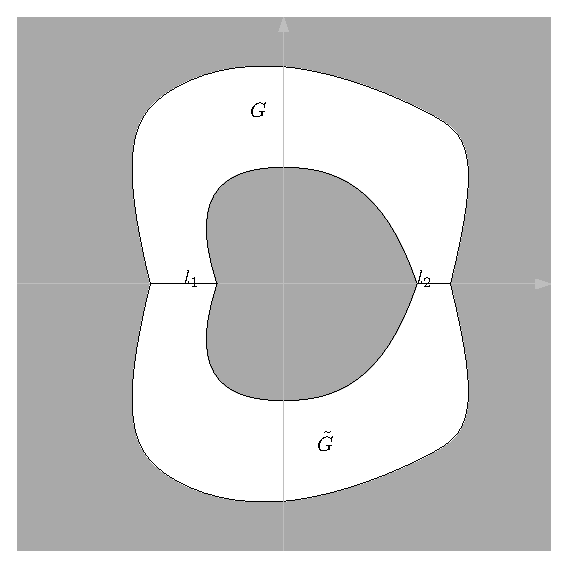
\includegraphics[scale=0.75]{1st.eps}
    \end{minipage}
    \begin{minipage}[c]{0.5\textwidth}
        \centering
        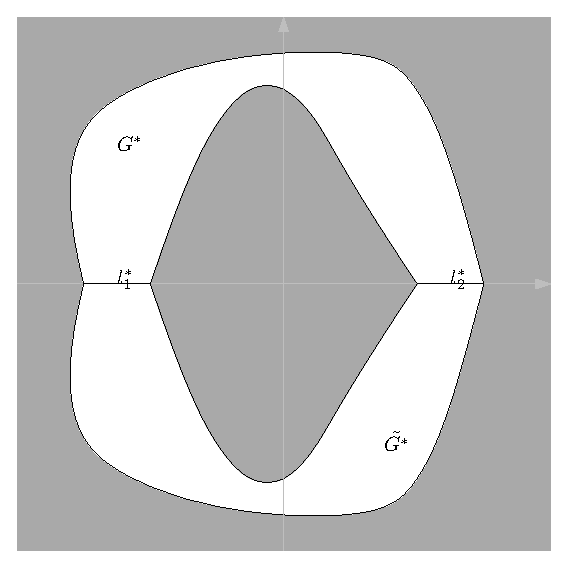
\includegraphics[scale=0.75]{2nd.eps}
    \end{minipage}
    \label{fig:25.1}
\end{figure}
\pr
Зададим функцию $F$ (искомое продолжение).
\begin{equation}\label{(25.1)}
    F(z) = \begin{cases}
        f(z), \ z \in G \cup \bigcup_{s=1}^n l_s \\
        \ol{f(\ol{z})}, \ z \in \tilde{G}
    \end{cases}
\end{equation}
Докажем дифференцируемость. Пусть $z_0 \in \tilde{G}$; тогда
\begin{align*}
  & \exists \varepsilon > 0: \ \forall \Delta z: \ \left| \Delta z \right| < \varepsilon \ z_0+\Delta z \in G
\end{align*}
\begin{align*}
  & \frac{F(z_0+\Delta z) - F(z_0)}{\Delta z} = \frac{\ol{f}(\ol{z_0+\Delta z}) - \ol{f}(\ol{z_0})}{\Delta z} = \ol{\frac{f(\ol{z_0}+\ol{\Delta z}) - f(\ol{z_0})}{\ol{\Delta z}}}
\end{align*}
Тогда
\begin{align*}
  & \ol{z_0} \in G, \ \ol{z_0} +\ol{\Delta z} \in G, \ \exists f'(\ol{z_0}) = \lim_{\Delta z \to 0} \frac{f(\ol{z_0}+\ol{\Delta z}) - f(\ol{z_0})}{\ol{\Delta z}}
\end{align*}
\begin{align*}
  & \exists F'(z_0) = \ol{f'(\ol{z_0})}
\end{align*}
Пусть теперь $x_0 \in l_s$. Докажем, что $F(z)$ непрерывна в $x_0$. Рассмотрим
нижний полукруг окрестности.
\begin{align*}
  & \lim_{z \os{\tilde{G}}{\to} x_0}F(z) = \lim_{\ol{z} \os{G}{\to} x_0}\ol{f(\ol{z})} = \ol{\lim_{\ol{z} \os{G}{\to} x_0}f(\ol{z})} = \ol{f(x_0)} = f(x_0) \in l_s^*
\end{align*}
Аналогично находится предел по верхнему полукругу.
\\
Тогда по теореме о стирании разреза $F(z)$ регулярна в $x_0$ и, значит,
регулярна во всей объединенной области.
\\
Докажем, наконец, однолистность. Область $G$ отображалась однолистно, как и
интервалы; каждая точка $\tilde{G}$ соответствует единственной точке $G$, как и
$\tilde{G^*}$ и $G^*$, а значит, отображение однолистно и на оставшейся части.
\corollary
принцип симметрии можнообобщить на симметрии относительно любой прямой или
окружности.
\pr
Всякую такую кривую можем перевести в действительную ось (область~--- в верхнюю
полуплоскость), применить принцип симметрии и перевести обратно.
\Example
Найти преобразование, переводящее данные области.
\begin{figure}[h!]
    \begin{minipage}[c]{0.45\textwidth}
        \centering
        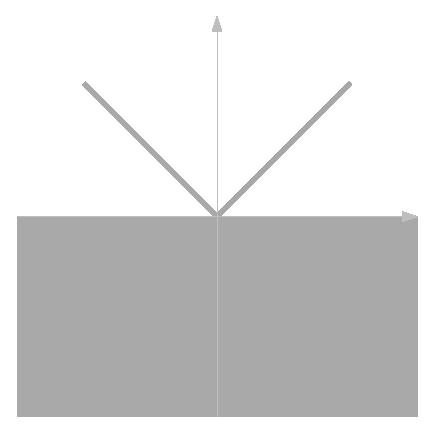
\includegraphics[scale=0.75]{ex24_1.eps}
    \end{minipage}
    \begin{minipage}[c]{0.1\textwidth}
        \centering
        \LARGE{$\mapsto$}
    \end{minipage}
    \begin{minipage}[c]{0.45\textwidth}
        \centering
        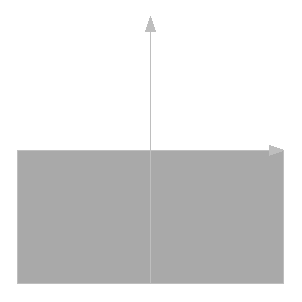
\includegraphics[scale=0.5]{half_plane.eps}
    \end{minipage}
    \label{fig:25.1}
\end{figure}
Воспользовавшись принципом симметрии, рассмотрим лишь правую часть вместе с
мнимой осью. Используя $w_1 = z^4$, получим $\CC \setminus[-4;+\infty)$, причем
функция будет непрерывно продлена на нижний край разреза от нуля и до
бесконечности. Применяя $w_2 = w_1+4$, получим $\CC \setminus[0;+\infty)$, причем
функция будет непрерывно продлена на нижний край разреза от $4$ и до
бесконечности. При помощи $w_3 = \sqrt{\left| w_2 \right|}\exp \left(
\dst \frac{i}{2}\argt w_2\right)$ получаем верхнюю полуплоскость, а $(-\infty;
-2]$ имеет непрерывное продолжение функции на себе. Затем сдвигаем этот разрез:
$w_4 = w_3+2$, и извлекаем корень: $w_5 = \sqrt{\left| w_4 \right|}\exp \left(
    \dst \frac{i}{2}\argt w_4\right)$. По принципу симметрии можем раскрыть все
до полуплоскости.
\begin{center}
    \begin{tabular}{cccc}
      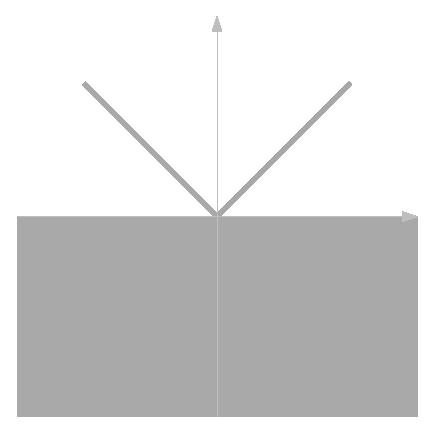
\includegraphics[scale=0.75]{ex24_1.eps} & $\Rightarrow$ & 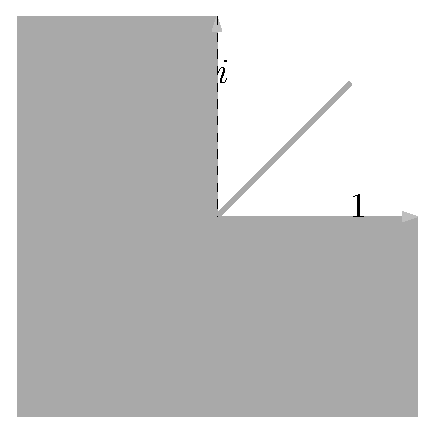
\includegraphics[scale=0.75]{2511.eps} & $\mapsto$ \\
    \end{tabular}
\end{center}
\begin{center}
    \begin{tabular}{cccc}
      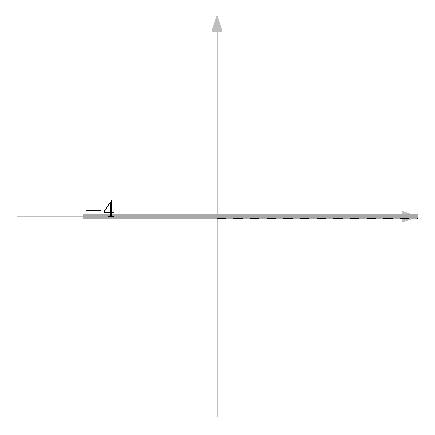
\includegraphics[scale=0.75]{2512.eps} & $\mapsto$ & 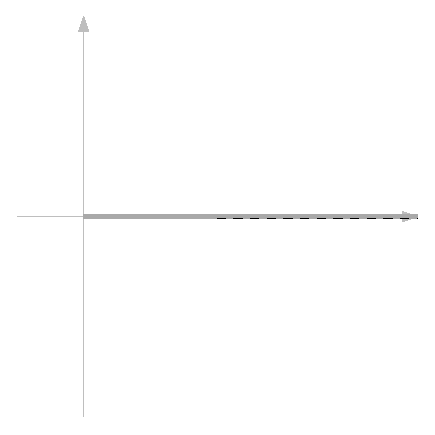
\includegraphics[scale=0.75]{2513.eps} & $\mapsto$ \\
    \end{tabular}
\end{center}
\begin{center}
    \begin{tabular}{cccc}
      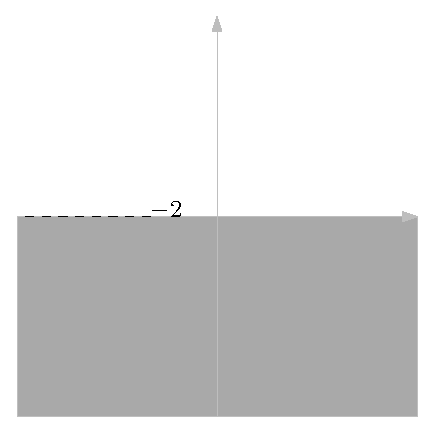
\includegraphics[scale=0.75]{2514.eps} & $\mapsto$ & 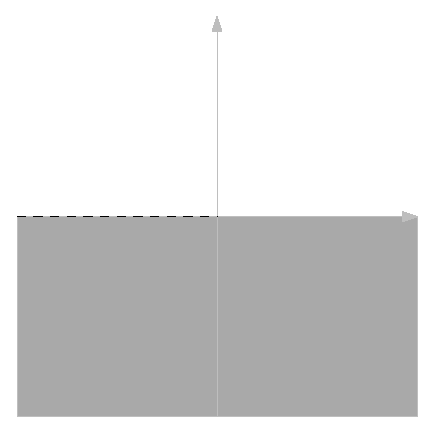
\includegraphics[scale=0.75]{2515.eps} & $\mapsto$ \\
    \end{tabular}
\end{center}
\begin{center}
    \begin{tabular}{cccc}
      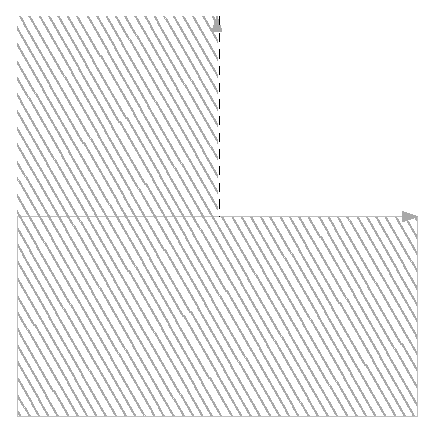
\includegraphics[scale=0.75]{2516.eps} & $\Rightarrow$ & 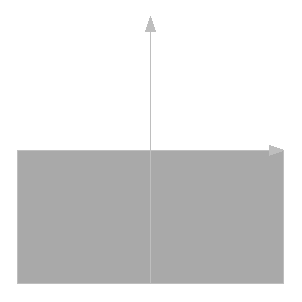
\includegraphics[scale=1]{half_plane.eps} & \\
    \end{tabular}
\end{center}
\Example
Найти преобразование, переводящее данные области.
\begin{align*}
  & G = \left\{ z = x+iy \mid y^2 < 2p \left( x+\frac{p}{2} \right) \right\}, \ p > 0
\end{align*}
\begin{figure}[h!]
    \begin{minipage}[c]{0.45\textwidth}
        \centering
        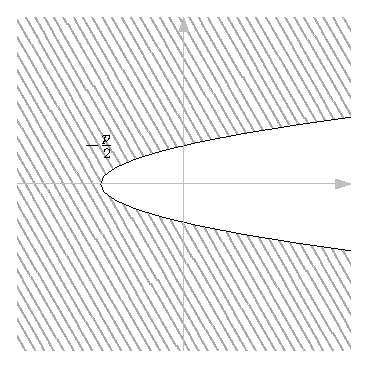
\includegraphics[scale=0.75]{2520.eps}
    \end{minipage}
    \begin{minipage}[c]{0.1\textwidth}
        \centering
        \LARGE{$\mapsto$}
    \end{minipage}
    \begin{minipage}[c]{0.45\textwidth}
        \centering
        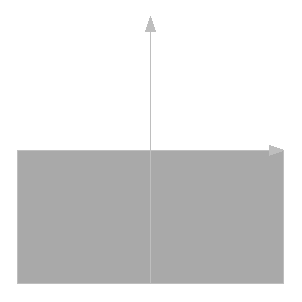
\includegraphics[scale=0.5]{half_plane.eps}
    \end{minipage}
    \label{fig:25.1}
\end{figure}
Воспользовавшись принципом симметрии, рассмотрим лишь верхнюю часть вместе с
действительной осью. Используя $w_1 = \sqrt{\left| z \right|}\exp \left(\dst
    \frac{i}{2}\argt z\right)$, получаем полуполосу. Растянем эту полуполосу при
помощи $w_2 = \pi\sqrt{\frac{2}{\pi}}$, экспонентой $w_3 = e^{w_2}$ превратим в
верхнюю полуплоскость с вырезанным единичным полукругом. Функцией Жуковского
$w_4 = dst \frac{1}{2}\left( w_3+\dst\frac{1}{w_4} \right)$ переводим в верхнюю
полуплоскость, но она имеет особый участок $[-1;+\infty)$. По принципу симметрии
можем раскрыть это до плоскости с разрезом по $(-\infty;-1]$, и легко, сдвигая
$w_5 = -w_4+1$ и извлекая корень $w_6 = \sqrt{\left| w_5 \right|}\exp \left(\dst
    \frac{i}{2}\argt w_5\right)$, получаем искомое.
\begin{center}
    \begin{tabular}{cccc}
      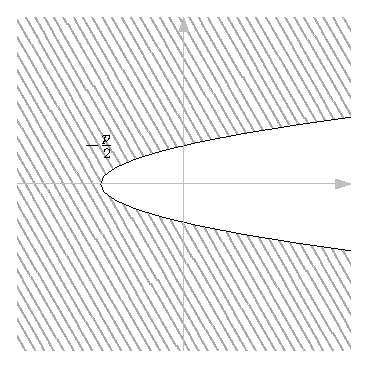
\includegraphics[scale=0.75]{2520.eps} & $\Rightarrow$ & 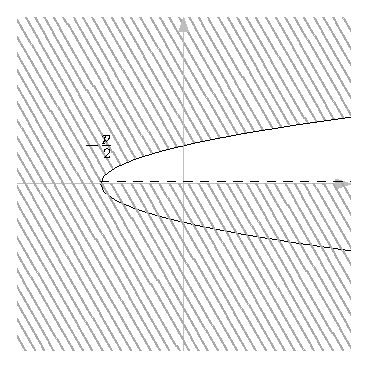
\includegraphics[scale=0.75]{2521.eps} & $\mapsto$ \\
    \end{tabular}
\end{center}
\begin{center}
    \begin{tabular}{cccc}
      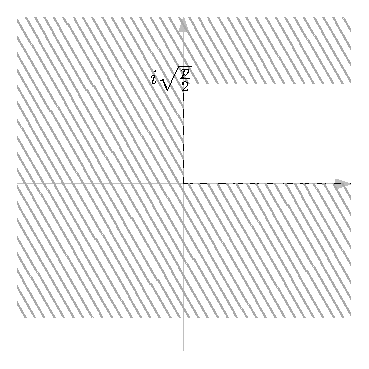
\includegraphics[scale=0.75]{2522.eps} & $\mapsto$ & 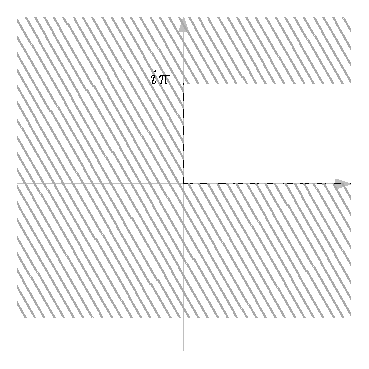
\includegraphics[scale=0.75]{2523.eps} & $\mapsto$ \\
    \end{tabular}
\end{center}
\begin{center}
    \begin{tabular}{cccc}
      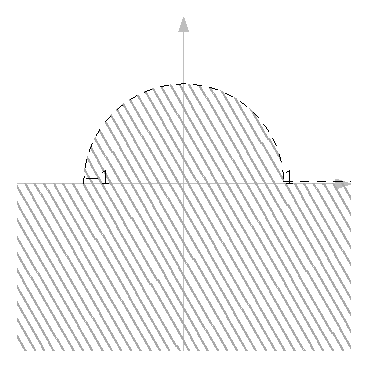
\includegraphics[scale=0.75]{2524.eps} & $\mapsto$ & 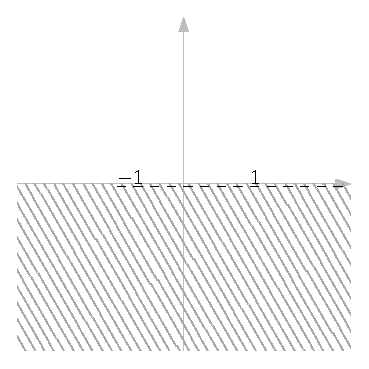
\includegraphics[scale=0.75]{2525.eps} & $\Rightarrow$ \\
    \end{tabular}
\end{center}
\begin{center}
    \begin{tabular}{cccc}
      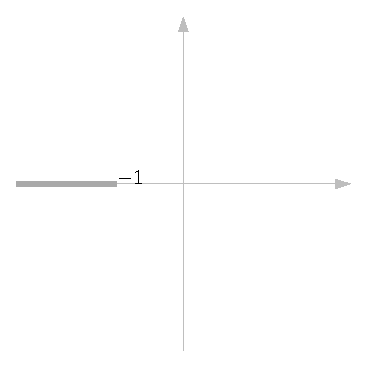
\includegraphics[scale=0.75]{2526.eps} & $\mapsto$ & 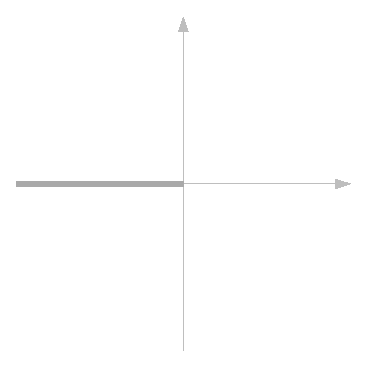
\includegraphics[scale=1]{2527.eps} & $\mapsto$ \\
    \end{tabular}
\end{center}
\begin{center}
    \begin{tabular}{cccc}
      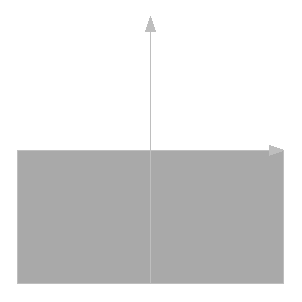
\includegraphics[scale=0.5]{half_plane.eps} & & & \\
    \end{tabular}
\end{center}
\section{$\S 26.$ Задача Дирихле на плоскости.}
\theorem
Пусть $f: G \mapsto D$ регулярная и непрстоянная. Пусть $\tilde{u}: D \mapsto
\RR$ гармоническая. Тогда $u(z) = \tilde{u}(f(z))$ также гармоническая.
\pr
Пусть $z_0 \in G$~--- произвольная точка. Пусть $f(z_0) = w_0$, и $f(G) =
G^*$~--- также, как известно, область. Тогда
\begin{align*}
  & \exists \varepsilon > 0: B_\varepsilon(w_0) \subseteq G^* \subseteq D
\end{align*}
По теореме $2$ $\S 4$
\begin{align*}
  & \exists h(w): \ \Real h(w) = \tilde{u}(w), \ w \in B_\varepsilon(w_0)
\end{align*}
причем $h$~--- регулярная. Рассмотрим теперь $h(f(z))$ в окрестности
$B_\delta(w_0)$, такой, чо $f\left( B_\delta(z_0) \right) \subseteq
B_\varepsilon(w_0)$. Тогда в этой окрестности $h$ будет регулярной,
$\tilde{u}(w) = \Real h(w)$~--- гармонической, тогда и $u(z) = \tilde{u}(f(z))$
тоже будет гармонической в этой окрестности, а в силу произвольности выбора
$z_0$~--- и на всей области.
\Def
\textbf{Классическим решением задачи Дирихле в области $G$} называется
следующее:
\begin{itemize}
    \item $G$~--- ограниченная односвязная область в $\CC$ с кучочно гладкой
    границей $\Gamma$;
    \item дана непрерывная функция $u_0(z)$ на этой границе;
    \item нужно найти гармоническую функцию $u(z)$ в области $G$, непрерывную на
    ее замыкании и удовлетворяющую условию: $u\Big|_\Gamma = u_0$.
\end{itemize}
\Def
\textbf{Общей задачей Дирихле} называется следующее:
\begin{itemize}
    \item $G$~--- односвязная область в $\CCC$ с кучочно гладкой границей $\Gamma$;
    \item дана непрерывная функция всюду за исключением коненого числа точек
    разрыва $1$ рода $\zeta_1, \dots, \zeta_n$ $u_0(z)$ на этой границе и
    ограниченная на ней за вычетом этих точек;
    \item нужно найти гармоническую функцию $u(z)$ в области $G$, ограниченную
    на ее замыкании, непрерывную на ее замыкании за вычетом этих точек и
    удовлетворяющую условию: $u = u_0$ на границе за вычетом этих точек.
\end{itemize}
\lemma
Лемма доказывается для случая ограниченной области.
\\
Пусть $G$~--- ограниченная односвязная область в $\CC$. Если решение общей
задачи Дирихле существует в этой области с $u_0(z)$ и $\tilde{\Gamma} = \Gamma
\setminus \dst \bigcup_{k=1}^n \left\{ \zeta_k \right\}$, то все значения $u(z)$
лежат на отрезке $\left[ m, M \right]$, где $m = \us{z \in\tilde{\Gamma}}{\inf} u_0(z)$, $M = \us{z \in\tilde{\Gamma}}{\sup}u_0(z)$.
\pr
Пусть $d = \sup \left| z_1-z_2 \right|$, $z_1, z_2 \in G$~--- диаметр множества.
Пусть
\begin{equation}\label{(26.1)}
    U_\varepsilon = M + \varepsilon \sum_{k=1}^n \ln \frac{d}{\left| z-\zeta_k\right|}, \ \varepsilon > 0
\end{equation}
Это гармоническая функция, причем она не меньше $M$ и непрерывна на замыкании
за вычетом точек разрыва, причем
\begin{equation}\label{(26.2)}
    \lim_{z \to \zeta_k} U_\varepsilon(z) = \infty
\end{equation}
Полагая
\begin{align*}
  & \gamma_r^k = \left\{ z \in G: \left| z - \zeta_k \right| = r\right\}
\end{align*}
\begin{equation}\label{(26.3)}
    \lim_{r \to 0}\min \left\{ U_\varepsilon(z) \mid z \in \gamma_r^k \right\} = +\infty
\end{equation}
\begin{align*}
    & \forall z \in \tilde{\Gamma} \ U_\varepsilon(z) > M\geq u_0(z) = u(z)
\end{align*}
Из ограниенности и выполнимости \eqref{(26.3)} для $u(z)$ имеем, чтопри
достаточно малых $r$ на границе области $G_r = G \setminus \dst \bigcup_{k=1}^n
B_r(\zeta_k)$ $U_\varepsilon(z) > U(z)$. По принципу максмума гармонической
функции это соотношение верно и для всей $G_r$.
\\
Фиксируем произвольную  $z \in G$. тогда $\exists r_0: z \in G_{r_0}$, значит,
$U_\varepsilon(z) > u(z)$ на всей $G$. При устремлении $\varepsilon$ к нулю
получаем, что $u(z) \leq M$.
\\
Аналогично можем ограничить сверху гармоническую $-u(z)$ числом $-m$ и получить
искомое.
\Note
Без условия ограниченности области лемма также справедлива.
\corollary
Для случая непостоянной $u_0(z)$ выполняются строгие неравенства.
\pr
От противного: предположим существование внутренней точки области, где $M$
достигается; тогда должна существовать $z_1 \in G: \ u(z_1) > M$ (аналогичнно
доказательству принципа максимума). Противоречие с неравенством, даже нестрогим.    
